\documentclass[12pt]{article}

\usepackage[a4paper,margin=1in]{geometry}
\usepackage{amsmath,amssymb,amsthm}
\usepackage{graphicx}
\usepackage{booktabs}
\usepackage{enumitem}
\usepackage{hyperref}
\usepackage{xcolor}
\setlength{\emergencystretch}{2em}

\hypersetup{
  colorlinks=true,
  linkcolor=blue!50!black,
  citecolor=blue!50!black,
  urlcolor=blue!50!black
}

\newtheorem{definition}{Definition}
\newtheorem{postulate}{Postulate}
\newtheorem{proposition}{Proposition}
\newtheorem{lemma}{Lemma}
\newtheorem{conjecture}{Conjecture}

\newcommand{\T}{\mathcal T}
\newcommand{\Ssrc}{\mathcal S}
\newcommand{\Rtau}{R_{\tau}}
\newcommand{\Ui}{U_i}
\newcommand{\Mta}{M_{\tau}}
\newcommand{\Obs}{\mathcal O}
\newcommand{\Def}{\mathcal D}
\newcommand{\Rel}{\mathcal J}
\newcommand{\Null}{\mathcal N}
\newcommand{\Ker}{\operatorname{Ker}}
\newcommand{\im}{\operatorname{im}}

\title{\textbf{Tau Core: An Atemporal Morphological Readout Framework for Emergent Physical Dynamics}\\
\large Foundation Paper I}
\author{Jozsef Olcsak\\
\small Independent researcher\\
\small AI-assisted theoretical-physics research workflow}
\date{Draft v0.1 --- 2026}

\begin{document}

\maketitle

\begin{abstract}
Tau Core is proposed here as a cautious foundation framework rather than a
completed physical theory.  Its starting point is the possibility that
ordinary dynamical physics is not fundamentally time evolution on a primitive
spacetime, but an effective readout of a deeper atemporal response structure.
The paper introduces a minimal formal spine
\[
  s \longmapsto \Rtau(s) \longmapsto U_i(\Rtau(s)),
\]
where \(s\) is a parent-side seed, \(\Rtau(s)\) is an endpoint-blind Tau
response, and \(U_i\) are sector readouts such as spacetime, observer-time,
quantum, gravitational, or mass/source readouts.  The central claim is not that
Tau Core is empirically validated, but that this readout architecture gives a
precise language for separating definitions, postulates, conditional
theorems, toy mechanisms, and future empirical tests.  We distinguish the
framework from block-universe ontology and from ordinary spacetime field
theory, define the Tau-side morphological body, formulate seven foundation
postulates, introduce readout-relative hidden defects via relift failure, and
give a finite toy model showing how one parent response can generate different
effective descriptions under different readouts.  The manuscript also records
the main blockers: the paper does not derive general relativity, quantum
mechanics, the Born rule, quantum field theory, the Standard Model, dark
matter, dark energy, or a physical parent action.  It is a position paper and
formal conjecture scaffold intended to make the Tau Core research program
discussable without promoting it to a completed theory.
\end{abstract}

\tableofcontents

\section{Purpose and claim boundary}

This manuscript is the first Roman-numbered Tau Core foundation paper.  It is
separate from the Arabic-numbered Tau Core paper sequence, where the latter is
used for bounded empirical or protocol packages.  The purpose here is more
basic: to state the current foundation language in a form that can be
criticized, compared, and refined.

The claim boundary is deliberately narrow.  The paper proposes a formal
architecture.  It does not claim empirical validation.  It does not derive
general relativity.  It does not derive quantum mechanics.  It does not
replace \(\Lambda\)CDM.  It does not solve the measurement problem, the dark
sector, neutrino physics, or the Standard Model.  It gives a vocabulary in
which those later questions can be stated without assuming that spacetime time
evolution is the primitive level.

The central idea can be written in one line:
\begin{equation}
  s \longmapsto \Rtau(s) \longmapsto U_i(\Rtau(s)).
  \label{eq:core-spine}
\end{equation}
The first arrow is not time evolution.  It is a parent-side response relation.
The second arrow is a readout.  A physical theory appears only after a readout
has supplied a codomain, a null policy, a closure test, and a validation
boundary.

\begin{figure}[t]
  \centering
  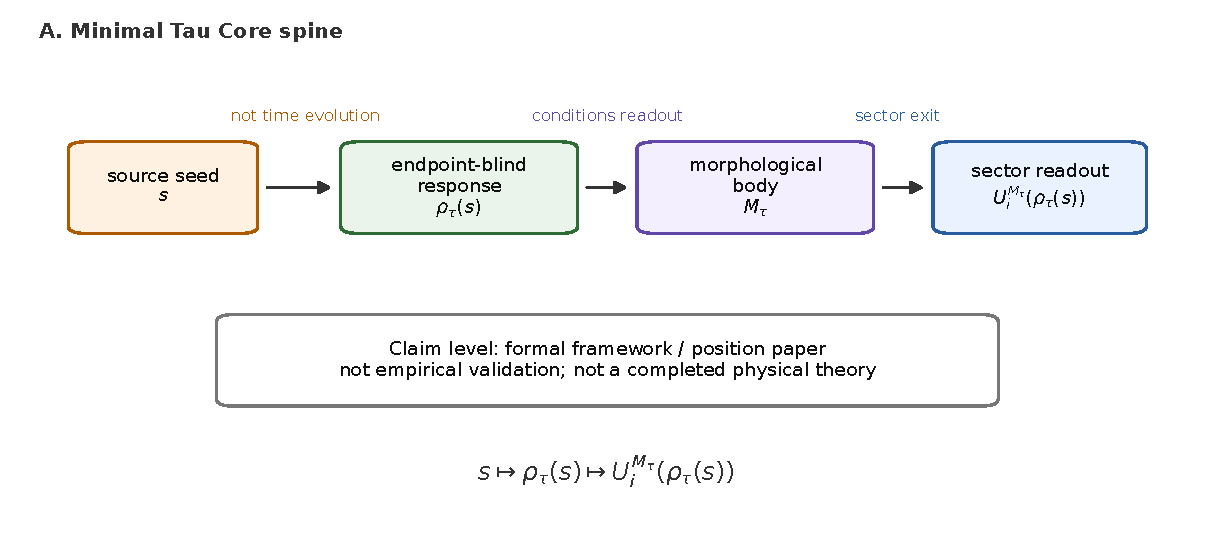
\includegraphics[width=0.95\linewidth]{figures/fig_core_spine.pdf}
  \caption{The minimal Tau Core spine used in Foundation Paper I.  A
  parent-side seed \(s\) induces an endpoint-blind Tau response
  \(\Rtau(s)\).  A Tau-side morphological body \(\Mta\) conditions sector
  readouts \(U_i\).  This is a formal architecture, not empirical validation.}
  \label{fig:core-spine}
\end{figure}

This paper is therefore closer to a formal conjecture paper or a position
paper than to a phenomenology paper.  It is useful only if it makes the
research program more falsifiable later.  A broad ontology that cannot be
turned into frozen source rules, null tests, or endpoint-blind predictions is
not useful as physics.  The framework below is written with that constraint in
mind.

\section{Why a foundation paper is needed}

Several themes in modern foundations already question whether time, spacetime,
or local dynamics should be primitive.  Canonical quantum gravity contains the
well-known problem of time, where a timeless constraint equation can coexist
with effective dynamics \cite{WheelerDeWitt1967,Rovelli2004}.  Relational
time constructions show how dynamics can be described through correlations
rather than external evolution \cite{PageWootters1983}.  Timeless or
configuration-space views have also been explored philosophically and
mathematically \cite{Barbour1999}.  Quantum reconstruction programs show that
large parts of quantum formalism can be organized by operational principles
rather than simply postulated \cite{Hardy2001,Chiribella2011,MasanesMueller2011}.

Tau Core does not claim to solve those programs.  It uses a different
organizing question:
\begin{quote}
Can physical sectors be treated as readouts of a deeper parent response, so
that time evolution, quantum state, gravity, mass, and observer-time are
effective sector descriptions rather than primitive categories?
\end{quote}
This question is intentionally broader than any one branch.  If it is too
broad, it becomes metaphysics.  The purpose of the present paper is to prevent
that drift by specifying the minimal objects that must exist before a Tau Core
statement becomes mathematically meaningful.

The immediate motivation is the following tension.  Many physical descriptions
use variables that are defined only after an observer, a section, a clock, a
measurement basis, or a spacetime background is in place.  But the same
description often treats those variables as if they were primitive.  Tau Core
instead separates:
\[
  \text{parent response}
  \quad \text{from} \quad
  \text{sector readout}.
\]
That separation is the entire point of Eq.~\eqref{eq:core-spine}.

\section{The name Tau Core}

The name ``Tau Core'' is historical.  The program began from a time-based
intuition: perhaps the time seen by a four-dimensional observer is not a
primitive background, but a projected response.  This explains the use of
\(\tau\), a symbol often associated with time or proper time in physics.

In the present architecture, however, \(\tau\) does not mean ordinary time.  It
names the parent-state side of the theory.  Time is one possible readout from
that side.  The distinction is important:
\begin{center}
\begin{tabular}{lll}
\toprule
Symbol or phrase & Meaning here & Not claimed here\\
\midrule
\(\tau\) & parent-state side & ordinary time itself\\
\(X_{\tau}\) & parent Tau state & detected physical field\\
\(\Rtau(s)\) & endpoint-blind response & time evolution\\
\(U_{\rm time}\) & time readout & derived clock theory\\
\(\Mta\) & morphological body & observed 4D shape\\
\bottomrule
\end{tabular}
\end{center}

Thus the theory is time-motivated but not time-reductionist.  It does not say
that everything is made of time.  It says that time belongs to the readout
side, while \(\tau\) names the deeper side from which time and other physical
sectors may be read.

\section{Difference from a block universe}

A block-universe reading treats a four-dimensional spacetime history as the
final object.  The comparison target is not a straw man.  The relativistic
background begins with Minkowski's four-dimensional spacetime formulation
\cite{Minkowski1909}.  The Rietdijk--Putnam--Maxwell line of argument then
uses relativity of simultaneity to motivate four-dimensionalism or eternalism
\cite{Rietdijk1966,Putnam1967,Maxwell1985,Thyssen2023RPM}.  Standard
surveys of the philosophy of spacetime and time describe the resulting
debates around being, becoming, eternalism, and the block universe
\cite{Savitt2021,MarkosianSullivan2025,PetersonSilberstein2010,Thyssen2020}.
In that setting one may summarize the block-universe reading as
\begin{equation}
  \text{Reality} = M_{4D}.
\end{equation}
Tau Core instead treats a four-dimensional block, when such a block is a good
description, as a readout:
\begin{equation}
  M_{4D} = U_{4D}(\Rtau(s)).
  \label{eq:block-readout}
\end{equation}
The difference is not cosmetic.  In a block-universe view the four-dimensional
object is the final arena.  In Tau Core it is an arena produced by a readout.
The parent response can in principle have distinctions that one readout
identifies, another ignores, and a third translates into effective dynamics.

This distinction also clarifies why Tau Core is not simply another form of
eternalism.  It can be compatible with an effective 4D block where that
description works, but it does not take the block as ontologically final.
Nor does the paper refute the block-universe literature.  It relocates the
four-dimensional block from final ontology to sector output:
\[
  \text{block as final object}
  \quad \longrightarrow \quad
  \text{block as } U_{4D}\text{-readout}.
\]

\begin{figure}[t]
  \centering
  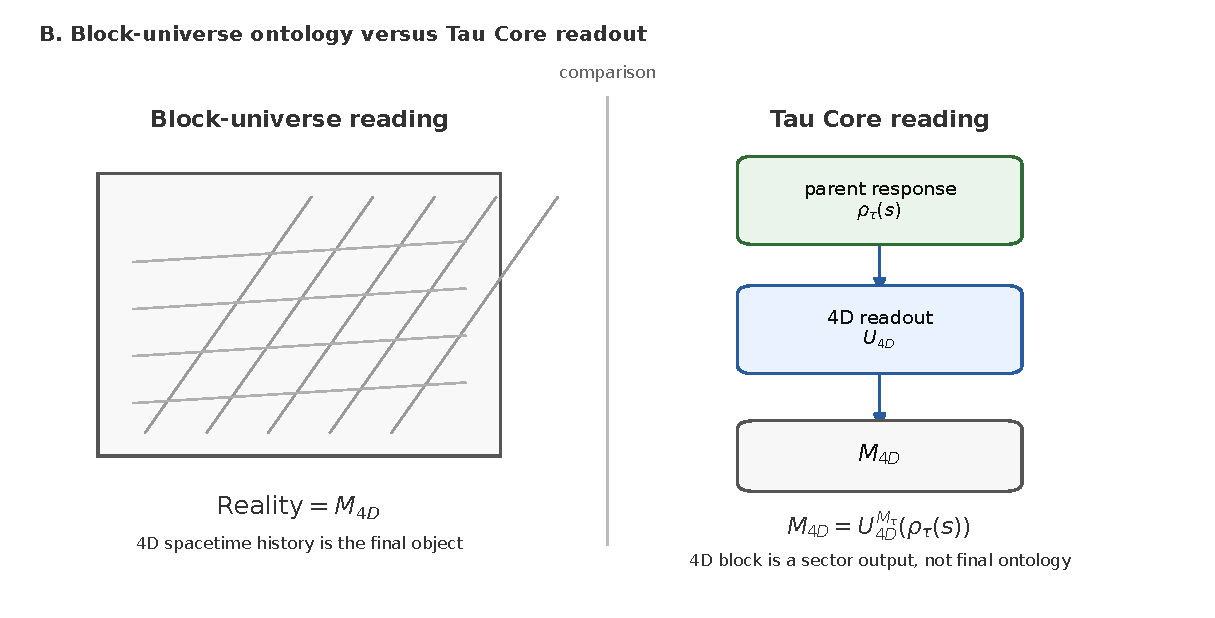
\includegraphics[width=0.95\linewidth]{figures/fig_block_vs_tau.pdf}
  \caption{The block-universe comparison used in this paper.  The left side
  represents the standard four-dimensional block reading, in which the
  spacetime history is the final object.  The right side represents the Tau
  Core position: the same effective 4D block may be a stable readout
  \(M_{4D}=U_{4D}(\Rtau(s))\) of a deeper parent response.  The figure is a
  conceptual distinction, not a proof against eternalism.}
  \label{fig:block-vs-tau}
\end{figure}

\section{Difference from ordinary spacetime field theory}

An ordinary field theory begins with a field on spacetime:
\begin{equation}
  \phi: M_{4D} \to V,
\end{equation}
and then studies the dynamics of \(\phi(x,t)\).  Tau Core rewrites the order:
\begin{equation}
  \phi_{\rm obs}(x,t)
  =
  U_{\phi}(\Rtau(s)).
  \label{eq:field-readout}
\end{equation}
The observed field is a readout.  The spacetime coordinates are also part of
the readout structure.  This does not make ordinary field theory wrong.  It
makes it effective: a very successful description after a particular sector
readout has become stable.

This is why Tau Core cannot claim physical success merely by writing a new
readout map.  To become physics, a readout must recover known limits and must
survive empirical controls.  If \(U_{\phi}\) is arbitrary, the framework is
empty.  The research program therefore needs source-frozen readout rules,
quotient-safe null policies, and explicit failure conditions.

\section{Core vocabulary}

\begin{definition}[Parent seed]
A parent seed \(s \in \Ssrc\) is a Tau-side source datum.  It is not an
observed endpoint and must not be chosen by looking at the endpoint residual
that a later readout is supposed to explain.
\end{definition}

\begin{definition}[Endpoint-blind Tau response]
An endpoint-blind Tau response is a map or relation
\[
  \Rtau: \Ssrc \to \mathcal R_{\tau}
\]
whose input is the parent seed and admissible parent-side constraints, not the
observational endpoint.  Endpoint blindness is a non-leakage rule, not a proof
that the response is physically real.
\end{definition}

\begin{definition}[Morphological body]
The Tau-side morphological body \(\Mta\) is the intrinsic structured body that
conditions readouts.  It is not an observed 4D morphology label.  It may carry
sector, branch, wall, null, Hessian-support, admissibility, history, and
observer/path-relevant structure.  A projected morphology is only a readout
handle on this deeper body.
\end{definition}

\begin{definition}[Readout]
A readout is a sector map
\[
  U_i : \mathcal R_{\tau} \to \Obs_i.
\]
The codomain \(\Obs_i\) may be a spacetime description, a time ordering, a
quantum access state, a gravitational response, a mass/source record, or a
more specialized observable structure.  Each readout has its own null
directions and validation boundary.
\end{definition}

\begin{definition}[Relift]
A relift for a readout \(U_i\) is a map or partial map
\[
  J_i : \Obs_i \to \mathcal R_{\tau}
\]
that attempts to reconstruct a parent-response representative from a readout
record.  It need not exist globally and need not be unique.
\end{definition}

\begin{definition}[Readout defect]
Given \(r=\Rtau(s)\), a readout defect is
\[
  h_i(r) = J_i(U_i(r)) - r,
  \label{eq:defect}
\]
whenever the subtraction is defined in a chosen linearized or quotient
representation.  More generally, the defect is the equivalence class of
failure of \(J_i U_i(r)\) to return the original parent-response
representative.
\end{definition}

Equation~\eqref{eq:defect} is not a dark-matter formula or a quantum-collapse
formula.  It is an abstract incompleteness record.  A physical branch must
later specify the codomain, quotient, units, known limits, and empirical test.

\section{Minimal readout calculus}

The formalism above is intentionally weak.  A readout is not yet a functor, a
field equation, a probability rule, or a variational principle.  Nevertheless,
some minimal calculus is needed if the framework is to avoid being only
language.

Let \(\mathcal R_{\tau}\) be a parent-response space and let \(U_i\) be a
readout.  The first mathematical object induced by a readout is its
indistinguishability relation:
\begin{equation}
  r \sim_i r'
  \quad \Longleftrightarrow \quad
  U_i(r)=U_i(r').
  \label{eq:readout-equivalence}
\end{equation}
This relation is readout-relative.  A distinction can be invisible to one
sector and visible to another.  In this sense, a readout is not just a map to
observables; it is also a rule for what counts as the same state for that
sector.

\begin{definition}[Readout kernel]
The readout kernel of \(U_i\) is the equivalence relation \(\sim_i\) defined
by Eq.~\eqref{eq:readout-equivalence}.  If \(\mathcal R_{\tau}\) has a linear
structure and \(U_i\) is linear, this reduces to the usual null space
\(\Ker U_i\).  In general it is an equivalence relation, not necessarily a
linear subspace.
\end{definition}

\begin{definition}[Readout refinement]
A readout \(U_j\) refines \(U_i\) if
\[
  r\sim_j r' \Longrightarrow r\sim_i r'.
\]
Equivalently, \(U_j\) distinguishes at least as much parent-response
information as \(U_i\).
\end{definition}

This gives a minimal partial order on readouts.  A more informative readout is
not automatically more physical.  It may be harder to stabilize, harder to
observe, or more vulnerable to noise.  But the refinement relation prevents
one from treating all readouts as interchangeable.

\begin{definition}[Joint readout]
Given readouts \(U_i\) and \(U_j\), the joint readout is
\[
  U_{ij}(r)=(U_i(r),U_j(r)).
\]
Its equivalence relation is the intersection:
\[
  \sim_{ij} \;=\; \sim_i \cap \sim_j.
\]
\end{definition}

\begin{proposition}[Joint readouts refine their components]
The joint readout \(U_{ij}\) refines both \(U_i\) and \(U_j\).
\end{proposition}

\begin{proof}
If \(r\sim_{ij}r'\), then \(U_i(r)=U_i(r')\) and \(U_j(r)=U_j(r')\).  Hence
\(r\sim_i r'\) and \(r\sim_j r'\).  Therefore the joint equivalence relation
is contained in each component equivalence relation.
\end{proof}

This trivial observation is one reason multi-readout tests are valuable.  If
two independent readout families point to the same parent-side distinction,
the candidate source class becomes more constrained.  But this also introduces
a warning: if the readouts are not independent, the joint readout may double
count the same source coordinate.  A mature Tau Core branch therefore needs a
source-overlap ledger.

\section{Nulls, quotients, and protected identity}

Every physical readout has null directions: changes in the parent response
that the readout treats as physically irrelevant.  Some nulls are ordinary
gauge redundancies.  Some are observational limitations.  Some are protected
identity relations: distinctions that should not be counted as physical
differences in a declared sector.

Let \(N_i\) denote the null relation for readout \(U_i\).  The quotient object
is written
\[
  [r]_i \in \mathcal R_{\tau}/N_i.
\]
The readout is quotient-safe only if
\[
  r N_i r' \Longrightarrow U_i(r)=U_i(r').
  \label{eq:quotient-safe}
\]
If Eq.~\eqref{eq:quotient-safe} fails, the readout assigns different
observables to parent states that it also declares physically equivalent.  Such
a readout is internally inconsistent.

The converse is not required.  A readout can identify more states than the
declared null relation identifies.  That is precisely readout loss.  The
important issue is whether the loss is allowed.  In empirical branches this is
handled by a source-freeze discipline: the readout-relevant source
coordinates must be declared before endpoint scoring.  In the foundation
branch this becomes a source-priority problem: the selected readout should not
erase protected source identity unless the erased distinction is explicitly
routed to the null quotient.

\begin{definition}[Protected source identity]
A protected source identity is an equivalence relation \(Q_{\rm src}\) on
parent-side seeds or source representatives that the theory treats as
source-level identity.  A readout rule is source-faithful if it does not
collapse distinct \(Q_{\rm src}\)-classes into one selected source class
without declaring the collapse as protected null structure.
\end{definition}

This definition is not an extra empirical claim.  It is a consistency demand.
Without it, a model can hide arbitrary distinctions in the parent space and
recover them only after seeing an endpoint.  That would make the theory
unfalsifiable.

\section{Endpoint blindness as a scientific rule}

Endpoint blindness is the operational face of the foundation idea.  A readout
model is endpoint-blind when the source, kernel family, amplitude rule, and
null policy are fixed before the target endpoint residual is inspected.

This is not a philosophical preference.  It is the only way a broad readout
framework can avoid becoming curve fitting.  If a galaxy rotation residual, a
cosmological distance residual, or a quantum outcome is used to choose the
source class that then explains it, the model has leaked the answer into its
input.

The minimal endpoint-blind record contains:
\begin{enumerate}[label=(E\arabic*)]
  \item a source object or source proxy;
  \item a declared readout family \(U_i\);
  \item a null and quotient policy;
  \item a source-overlap decision for all channels used together;
  \item a freeze artifact or equivalent timestamped declaration;
  \item forbidden endpoint fields;
  \item controls and failure conditions.
\end{enumerate}

Foundation Paper I does not run such an endpoint test.  It states why later
branches need it.  The philosophical content of Tau Core becomes scientific
only when it produces source-frozen rules that can fail.

\section{How effective dynamics appears}

Tau Core replaces primitive time evolution by readout-parametrized variation.
Let \(r=\Rtau(s)\) be atemporal at the parent-response level.  Suppose a
readout \(U_i\) produces a record that can be coordinatized by a parameter
\(t_i\):
\[
  U_i(r) = o_i(t_i).
\]
Then the derivative
\[
  \frac{d o_i}{dt_i}
\]
is meaningful inside the readout.  It need not correspond to a parent-time
derivative.  This is the minimal sense in which dynamics is emergent.

The distinction can be made sharper by considering two readouts of the same
parent response.  One readout may admit a temporal parameter \(t_A\), while
another admits a static relational record:
\[
  U_A(r)=o_A(t_A), \qquad U_B(r)=C_B.
\]
There is no contradiction.  The first readout organizes the parent response as
a time-indexed sequence.  The second organizes it as a correlation or
constraint.  A conventional physical theory may then choose the first
description because it is useful, local, and predictive.  Tau Core's claim is
weaker: usefulness of a temporal parameter does not make time primitive.

This is also why observer time must be sector-typed.  A clock used in a
galaxy-rotation analysis, a lensing time-delay analysis, a cosmological
distance analysis, and a quantum measurement protocol are not automatically
the same parent object.  They may share a local proper-time limit, but that
limit has to be earned.

\section{Toy model with effective time}

The finite model above can be extended to show effective time.  Let
\[
  r=(a_0,a_1,\ldots,a_n,c)\in \mathbb R^{n+2}.
\]
Define a readout
\[
  U_{\rm seq}(r) = (a_0,a_1,\ldots,a_n),
\]
and choose the index \(k\) as an effective time coordinate.  The readout sees
a sequence \(a_k\).  A finite-difference law can be defined:
\[
  \Delta a_k = a_{k+1}-a_k.
\]
Nothing in the parent object has evolved.  The parent response already
contains the indexed structure.  The readout has supplied an ordering and
therefore an effective dynamics.

Now define a second readout
\[
  U_{\rm sum}(r)=\sum_{k=0}^n a_k.
\]
This readout sees no time sequence, only an aggregate.  The hidden component
relative to \(U_{\rm sum}\) is the loss of ordered information.  The hidden
component relative to \(U_{\rm seq}\) includes \(c\).  Again, hiddenness is
readout-relative.

This toy model is deliberately too simple to be physics.  It only shows that
the sentence ``time is a readout'' can be made mathematically literal without
introducing backward causation or a second physical clock.

\begin{figure}[t]
  \centering
  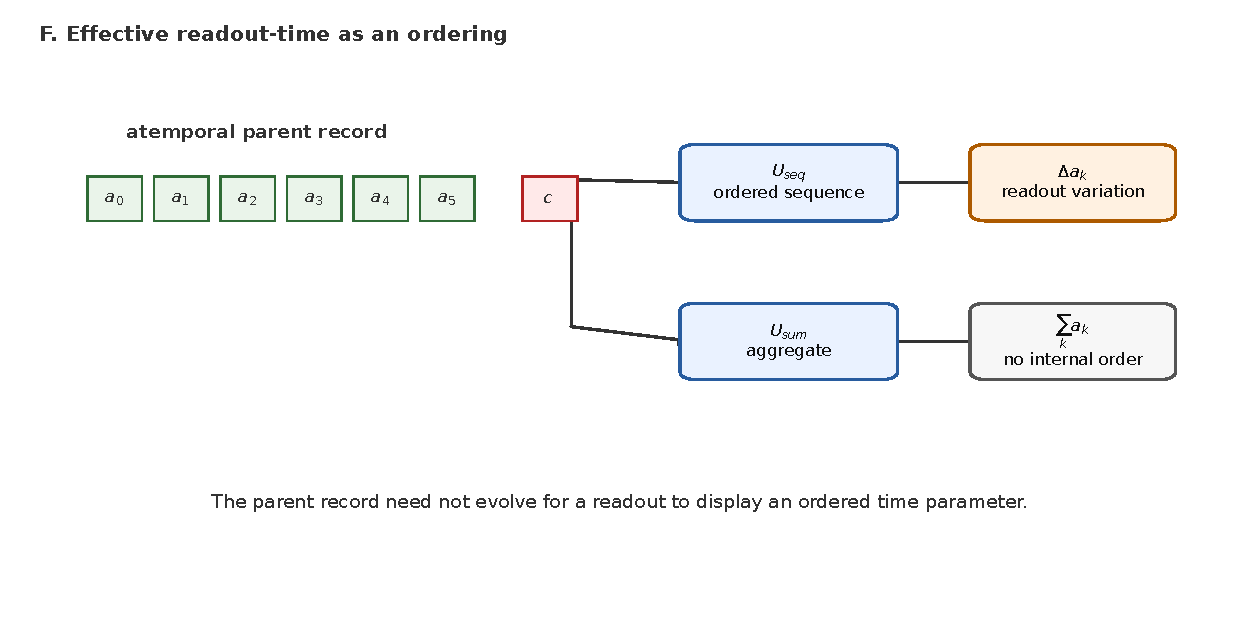
\includegraphics[width=0.95\linewidth]{figures/fig_effective_time_readout.pdf}
  \caption{A finite toy model for effective time.  The parent record is not
  itself evolving.  The sequence readout \(U_{\rm seq}\) exposes an ordered
  list and therefore supports finite differences \(\Delta a_k\).  The
  aggregate readout \(U_{\rm sum}\) exposes a different observable and loses
  the internal ordering.  Effective dynamics is therefore readout-relative in
  this model.}
  \label{fig:effective-time}
\end{figure}

\begin{figure}[t]
  \centering
  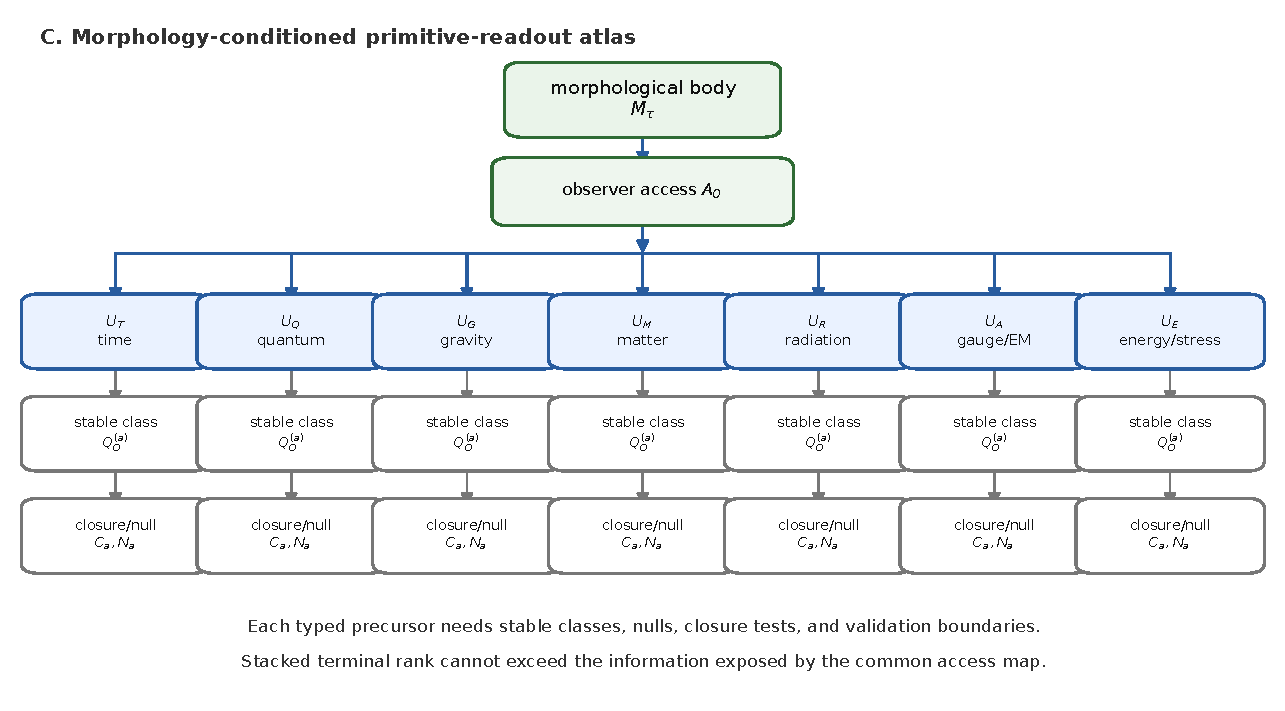
\includegraphics[width=0.95\linewidth]{figures/fig_readout_atlas.pdf}
  \caption{A parent response can have several sector readouts.  The same
  parent object may be read as spacetime, observer-time, quantum access,
  gravitational response, or mass/source structure.  Each sector requires its
  own codomain, null policy, closure test, and validation boundary.  The paper
  does not assume that these readouts are automatically additive or mutually
  complete.}
  \label{fig:readout-atlas}
\end{figure}

\section{Seven foundation postulates}

The postulates below are not proved in this paper.  They define the candidate
framework.  Later papers or theory notes may try to derive or weaken them.

\begin{postulate}[Tau substrate]
There exists a parent-level structure \(\T\) that is not, at the foundation
level, ordinary spacetime evolution.
\end{postulate}

\begin{postulate}[Seed-response]
Physical configurations are represented at the parent level by endpoint-blind
responses to seeds:
\[
  s \in \Ssrc, \qquad r=\Rtau(s)\in \mathcal R_{\tau}.
\]
\end{postulate}

\begin{postulate}[Endpoint blindness]
The response \(\Rtau(s)\), and any source object used to select a readout
kernel, must be specified without using the endpoint residual that the readout
is later asked to explain.
\end{postulate}

\begin{postulate}[Readout emergence]
Observed physical descriptions are sector readouts:
\[
  O_i = U_i(\Rtau(s)).
\]
Time, spacetime, quantum access, gravity, and mass/source descriptions are
readout candidates rather than primitive categories.
\end{postulate}

\begin{postulate}[Effective dynamics]
Time evolution appears only when a readout admits a stable ordering or clock
coordinate.  A derivative such as
\[
  \frac{d}{dt} U_i(\Rtau(s))
\]
is an effective readout derivative, not a primitive parent-time derivative.
\end{postulate}

\begin{postulate}[Hidden defect]
If a readout and its allowed relift fail to recover the parent-response
representative modulo the declared null relation, the non-reliftable component
is recorded as a hidden defect of that readout.
\end{postulate}

\begin{postulate}[Tension as readout failure]
Some observational or theoretical tensions may be modeled as readout,
closure, or relift defects.  This is a research hypothesis.  It becomes
physical only after source-frozen rules, controls, known limits, and held-out
tests are supplied.
\end{postulate}

\section{The claim ladder}

A central discipline of Tau Core is to separate claim levels.  The framework
contains definitions, postulates, conjectures, conditional theorems, toy
models, numerical evidence, and empirical validation.  These are not
interchangeable.

\begin{figure}[t]
  \centering
  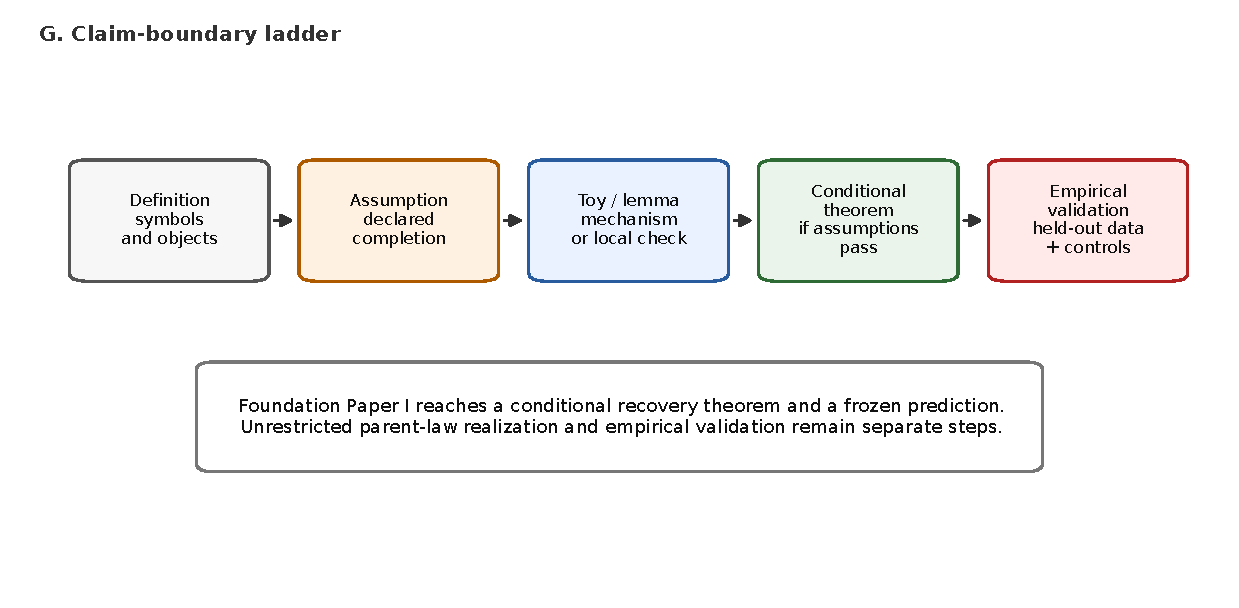
\includegraphics[width=0.95\linewidth]{figures/fig_claim_ladder.pdf}
  \caption{The claim ladder for Foundation Paper I.  The present manuscript
  stops at definitions, postulates, conditional implications, and toy
  mechanisms.  It does not claim empirical validation.}
  \label{fig:claim-ladder}
\end{figure}

The most common failure mode for broad foundation programs is promotion by
language: a metaphor becomes a mechanism, a mechanism becomes evidence, and
evidence becomes validation.  This paper avoids that promotion.  For example,
saying that observer-time is a readout does not derive a physical clock.
Saying that dark-sector language may be a hidden-defect language does not
remove dark matter.  Saying that quantum state may be a readout does not
derive Hilbert space.

\section{A finite toy model}

The following model is intentionally small.  Its role is not to reproduce
physics.  Its role is to show the readout logic without infinite formal
machinery.

Let the parent response space be
\[
  \mathcal R_{\tau} = \mathbb R^3,
  \qquad
  r=(a,b,c).
\]
Let two readouts be
\[
  U_A(a,b,c)=(a,b),
  \qquad
  U_B(a,b,c)=(a,c).
\]
These readouts forget different coordinates.  Choose canonical relifts
\[
  J_A(x,y)=(x,y,0),
  \qquad
  J_B(x,z)=(x,0,z).
\]
Then the readout defects are
\[
  h_A(r)=J_AU_A(r)-r=(0,0,-c),
\]
and
\[
  h_B(r)=J_BU_B(r)-r=(0,-b,0).
\]
The same parent response therefore has different hidden components under
different readouts.  There is no contradiction: each readout has a different
null policy.

\begin{proposition}[Readout-relative hidden component]
In the toy model above, a component hidden under readout \(U_A\) can be visible
under readout \(U_B\), and conversely.
\end{proposition}

\begin{proof}
The coordinate \(c\) is absent from \(U_A(a,b,c)\) and appears as the defect
\((0,0,-c)\) under the canonical relift \(J_A\).  The same coordinate is
present in \(U_B(a,b,c)\).  Similarly, \(b\) is visible under \(U_A\) and hidden
under \(U_B\).  Thus hiddenness is readout-relative.
\end{proof}

The lesson is small but important.  A hidden component is not necessarily a new
substance.  It may be a component that a chosen readout cannot relift.  Whether
this idea has anything to do with dark sectors, quantum measurement, or
cosmology is a later physical question.  The toy model only licenses the
logical grammar.

\begin{figure}[t]
  \centering
  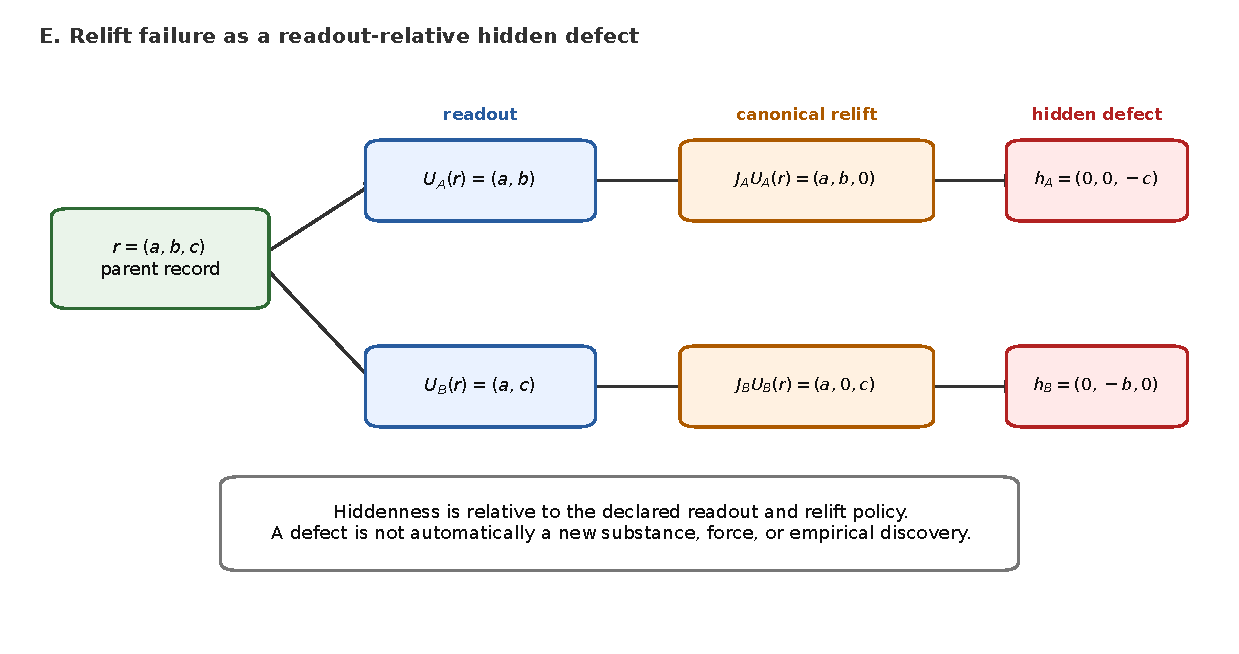
\includegraphics[width=0.95\linewidth]{figures/fig_hidden_defect.pdf}
  \caption{Readout-relative hidden defects.  Two readouts of the same parent
  response can have different relift failures.  A hidden component is not
  automatically a new force or substance; it is first an incompleteness record
  relative to a declared readout.}
  \label{fig:hidden-defect}
\end{figure}

\section{Morphological body versus projected morphology}

The phrase ``morphology'' can be misleading if left unqualified.  In ordinary
astronomical use it often means visible shape or catalogue type.  In Tau Core,
the primary object is not the observed shape.  It is the Tau-side
morphological body \(\Mta\).

The morphological body is the structured source object that conditions
readouts.  A galaxy image, a rotation curve, a cosmic-web tensor, a lensing
map, or a quantum measurement context can be a projected handle on the body,
but not the whole body.  This distinction became necessary because a single 4D
appearance can underdetermine the readout-relevant source.  For example, a
present projected shape may not contain enough information about history,
observer/path geometry, closure class, or null structure.

For Foundation Paper I, the minimal role of \(\Mta\) is:
\begin{equation}
  O_i = U_i[\Mta](\Rtau(s)).
  \label{eq:morph-conditioned}
\end{equation}
The bracket indicates that the readout map may depend on the morphological
body.  It does not say that \(\Mta\) has been physically derived.  It says that
readout selection is not source-free.

This point also prevents double counting.  If two proposed correction terms
use the same source coordinate, they should not be added independently unless
a source-side split justifies the separation.  Otherwise the readout model is
only relabeling the same source information twice.

\section{Observer time}

Tau Core treats observer time as a readout, not as a primitive parameter on the
parent side.  The schematic form is
\begin{equation}
  t_{\rm obs}^{S}
  =
  U_{\rm time}^{S}(\Rtau(s),\Mta,\mathcal O_S,\gamma_S),
  \label{eq:observer-time}
\end{equation}
where \(S\) is a sector, \(\mathcal O_S\) is observer-interface data, and
\(\gamma_S\) denotes path or section data relevant to that sector.

Equation~\eqref{eq:observer-time} is not a derived clock theory.  It is a
discipline rule.  It says that an observer's time belongs to the observer's
readout bundle.  A later physical theory must explain when
\(t_{\rm obs}^{S}\) reduces to proper time, when it admits corrections, and
how those corrections can be measured without circularity.

This also clarifies why future-directed or history-like terms in Tau Core
should not be read as backward causation.  They are components of a deeper
parent response whose different 4D readout slices may appear as past, present,
or future.  The parent object is not evolving in an external time.  The
observed ordering is created inside the readout.

\section{Quantum readout}

The quantum branch is one of the natural targets for the readout language, but
it is also one of the most dangerous places to overclaim.  A minimal quantum
readout might have the form
\begin{equation}
  q = U_q(\Rtau(s)),
\end{equation}
where \(q\) is an access-state or probability-assignment record.  But this is
far below deriving Hilbert space or the Born rule.

Existing reconstruction programs show that quantum theory can be approached
from information-theoretic or operational axioms.  Examples include
Hardy-style, purification-style, and local/reversible reconstruction routes
\cite{Hardy2001,Chiribella2011,MasanesMueller2011}.  Generalized
probabilistic and Jordan-algebraic routes clarify how much structure is needed
before Hilbert-space quantum theory is forced \cite{BarnumWilce2014}.  Tau
Core can use these results as boundary discipline.  It must not claim that a
finite contextual readout grammar already implies complex Hilbert space.

The current safe statement is:
\begin{quote}
If Tau Core supplies an ordered convex access-state space, separating effects,
an appropriate self-dualizing pairing, continuous homogeneous reversible
symmetry, composition rigidity, and trace uniqueness, then a Born/Hilbert
representation becomes a conditional target.
\end{quote}
This is a conditional reconstruction route, not a derivation.  The present
paper includes quantum readout only to show where it sits in the common
architecture.

\section{Gravity and dark-sector readouts}

The gravity branch motivates the hidden-defect vocabulary.  A gravitational
readout may fail to relift all source-relevant structure into a Newtonian,
relativistic, or closure-compatible description.  In abstract notation:
\begin{equation}
  h_g = J_g U_g(\Rtau(s)) - \Rtau(s).
\end{equation}
If a component of \(h_g\) survives the declared null quotient and has a
measurable 4D readout, it becomes a candidate residual channel.  This is still
not a dark-matter replacement.  It is a source of possible residual structure.

The same discipline applies to dark-sector language.  Tau Core may eventually
ask whether some dark-sector phenomena are better understood as
readout-relative hidden defects.  Foundation Paper I does not answer that
question.  It only defines the level at which the question becomes meaningful.
To make a dark-sector claim, one would need source-frozen kernels, conventional
baseline comparisons, covariance/systematics treatment, and failure criteria.

\section{Cosmological readout}

Cosmology is another natural readout target because the observed expansion
history, distance ladder, growth data, lensing data, and CMB inference are all
compressed through model-dependent readout assumptions.  A Tau Core
cosmological readout might be written
\begin{equation}
  O_{\rm cosmo}
  =
  U_{\rm cosmo}(\Rtau(s),\Mta^U,\gamma_{\rm path},\mathcal O_{\rm obs}),
\end{equation}
where \(\Mta^U\) is a universe-scale morphological body, \(\gamma_{\rm path}\)
is path/environment data, and \(\mathcal O_{\rm obs}\) is observer-interface
data.

Again, the notation is not a result.  It is a warning against compressing all
cosmological tensions into a single function of the scale factor.  A real
cosmological Tau Core branch would need multi-probe covariance, source-native
void/web/path/time channels, and a clear relation to \(\Lambda\)CDM limits.

\section{Relationship to the existing paper sequence}

The Arabic-numbered Tau Core papers are not required for the logic of this
foundation paper.  They are narrower, operational packages.  Some examine
galaxy residuals, some define source-frozen morphology or projection kernels,
some formulate dark-sector decision protocols, and some define cosmological or
web-witness audit ladders.  They are evidence-seeking packages, not proofs of
the parent ontology.

Foundation Paper I has the opposite role.  It defines the vocabulary that
those operational papers can later use.  It should not borrow their numerical
outcomes as proof.  A positive empirical audit in a later branch can motivate
the framework, but it does not validate the parent theory unless the path from
parent source to readout rule is itself frozen, non-circular, and tested.

This separation is important for scientific criticism.  A critic should be
able to reject a galaxy-kernel result without thereby rejecting the formal
readout architecture.  Conversely, a critic can reject the foundation
architecture while still accepting that a particular empirical paper performed
a reproducible audit.

\section{Comparison with adjacent ideas}

Tau Core overlaps in spirit with several families of ideas, but it should not
be confused with them.

\paragraph{Relational time.}
Relational-time approaches show how dynamics can be recovered through
correlations.  Tau Core agrees that external time need not be primitive, but it
places this inside a broader readout atlas.  Time is one readout among several,
not the only reconstruction target.

\paragraph{Shape dynamics and relational configuration.}
Shape-dynamics-inspired work emphasizes that spacetime structure may be
reformulated through different symmetry or relational choices
\cite{GomesKoslowski2012}.  Tau Core uses this as a cautionary analogy: one
must state which structure is primitive and which is recovered.  It does not
import shape dynamics as a proof.

\paragraph{Quantum reconstruction.}
Quantum reconstruction programs provide a model for turning operational
principles into formal structure.  Tau Core's quantum branch must meet a
similar standard.  It cannot derive Hilbert space merely by naming a quantum
readout.

\paragraph{Holography and error correction.}
Holographic quantum error correction shows that bulk-like structure can be
encoded and recovered nontrivially from boundary data
\cite{AlmheiriDongHarlow2015}.  Tau Core treats this as an analogy for
readout/reconstruction discipline, not as evidence for the Tau ontology.

\section{What would count as progress}

The framework becomes stronger only if abstract readout language is converted
into bounded tasks.  Examples include:
\begin{enumerate}[label=(\arabic*)]
  \item deriving a non-circular parent response law \(\Rtau\);
  \item defining a source-realizable morphological body \(\Mta\);
  \item proving that a readout map has a quotient-safe null policy;
  \item deriving a known physical limit, such as proper time or Newtonian
  gravity, as a controlled readout limit;
  \item producing source-frozen empirical rules that survive held-out tests;
  \item preserving negative results by demoting failed kernels instead of
  retuning them after endpoint inspection.
\end{enumerate}

The weakest useful form of progress is a toy model that exposes a blocker.  A
failed theorem can be valuable if it shows which extra principle is needed.
For example, local convexity or a positive Hessian may not force global
exposed-face duality; finite contextual grammars may not force Hilbert space;
and source stability may not force a unique source basis.  Such negative
results help keep the framework honest.

\section{Likely objections}

A foundation framework should be written so that criticism has handles.  We
therefore list several likely objections and the intended answer.

\paragraph{Objection 1: this is only a change of language.}
This objection is serious.  The framework is only useful if readout language
forces new constraints.  The minimum non-linguistic constraints are endpoint
blindness, null/quotient safety, source-overlap discipline, known-limit
recovery, and explicit failure conditions.  Without these, Tau Core would be a
vocabulary rather than a research program.

\paragraph{Objection 2: the parent response is unobservable.}
The parent response is not directly observed by assumption.  But this alone is
not fatal; many theoretical objects are inferred through constrained effects.
The relevant question is whether a declared readout rule produces predictions
or exclusions that could have failed.  If no such rule is produced, the parent
response remains a metaphysical placeholder.

\paragraph{Objection 3: the framework can explain anything.}
This is the most important danger.  Tau Core must therefore preserve negative
results.  A failed frozen kernel should be demoted, not retuned after looking
at the residual.  A wrong readout family should remain wrong.  A source class
that cannot be independently justified should not be promoted.  If the
framework always rescues itself by adding another projection, it fails as
science.

\paragraph{Objection 4: atemporal response sounds like a block universe.}
The difference is Eq.~\eqref{eq:block-readout}.  A block universe treats a 4D
history as the final object.  Tau Core treats a 4D history as one possible
readout.  The distinction matters only if other readouts impose independent
constraints.  If they do not, Tau Core collapses back into ordinary effective
description.

\paragraph{Objection 5: no physical law is derived.}
Correct.  Foundation Paper I does not derive a physical law.  It defines the
objects a later derivation must use.  A future physical law would require a
parent action or closure principle, a domain, a null policy, variation support,
units, calibration, and known limits.

\section{Minimal mathematical maturity checklist}

Before a branch of Tau Core should be treated as more than a toy model, it
should satisfy at least the following checklist.

\begin{center}
\begin{tabular}{p{0.28\linewidth}p{0.58\linewidth}}
\toprule
Requirement & Meaning\\
\midrule
Source declaration & The parent-side source or proxy is declared before endpoint scoring.\\
Readout codomain & The observable space \(\Obs_i\) is specified.\\
Null policy & Gauge, redundancy, and protected-null directions are declared.\\
Quotient safety & Equivalent parent representatives give the same readout.\\
Relift policy & The branch states whether and how \(J_i\) is defined.\\
Known limit & The readout recovers a standard limit where required.\\
Failure rule & Failed controls cause demotion, not post-hoc retuning.\\
\bottomrule
\end{tabular}
\end{center}

This checklist is intentionally weaker than a full physical theory.  It is
also stronger than a metaphor.  A branch that cannot fill these rows should not
be advertised as a physical result.

\section{The Roman foundation sequence}

This paper is the first member of a separate Roman-numbered foundation series.
It should not be confused with the Arabic-numbered empirical/protocol sequence.
The intended division is:
\[
\begin{array}{ll}
\text{Paper 1--14} & \text{bounded empirical or protocol packages},\\
\text{Foundation Paper I, II, ...} & \text{conceptual and mathematical foundation papers}.
\end{array}
\]

The proposed next papers are:
\begin{itemize}
  \item \textbf{Foundation Paper I}: atemporal morphological readout;
  framework only, with no physical validation claim.
  \item \textbf{Foundation Paper II}: quantum readout; no unconditional
  Hilbert, Born-rule, or QFT derivation claim.
  \item \textbf{Foundation Paper III}: hidden defects and dark sectors; no
  dark-matter or dark-energy replacement claim.
  \item \textbf{Foundation Paper IV}: observer-time and cosmology; no
  Hubble-tension or \(\Lambda\)CDM replacement claim.
  \item \textbf{Foundation Paper V}: flavor and neutrino readout; no
  neutrino-anomaly or Standard Model claim.
\end{itemize}

The purpose of this split is defensive in the good sense.  A foundation paper
can state a formal conjecture without pretending to be a data paper.  A data
paper can test a narrow rule without requiring acceptance of the full
ontology.  This separation makes both kinds of work easier to criticize.

\section{A compact formal summary}

The framework can be summarized as the following object package:
\[
  \mathfrak T
  =
  (\Ssrc,\mathcal R_{\tau},\Rtau,\Mta,\{U_i\},\{N_i\},\{J_i\}).
\]
Here \(\Ssrc\) is a seed/source domain, \(\mathcal R_{\tau}\) is a response
domain, \(\Rtau\) is the endpoint-blind response map or relation, \(\Mta\) is
the morphological body, \(U_i\) are readouts, \(N_i\) are null policies, and
\(J_i\) are optional relifts.

The minimal consistency conditions are:
\begin{align}
  &s \text{ is fixed without endpoint leakage},\\
  &r=\Rtau(s) \text{ is defined on the declared source domain},\\
  &r N_i r' \Rightarrow U_i(r)=U_i(r'),\\
  &h_i(r)=J_iU_i(r)-r \text{ is interpreted only modulo } N_i,\\
  &\text{known physical limits are recovered before physical promotion}.
\end{align}

The strongest claim of this paper is that \(\mathfrak T\) is a coherent
starting package for a readout-based research program.  It is not a proof that
Nature uses such a package.

\section{What is not proved}

For clarity, we list the main non-results.

\begin{itemize}
  \item The paper does not prove that the Tau substrate exists physically.
  \item The paper does not provide a parent action.
  \item The paper does not derive physical time.
  \item The paper does not derive general relativity.
  \item The paper does not derive quantum mechanics, the Born rule, collapse,
  or QFT.
  \item The paper does not derive the Standard Model.
  \item The paper does not explain neutrino physics.
  \item The paper does not eliminate dark matter or dark energy.
  \item The paper does not validate any empirical Tau Core claim.
\end{itemize}

These limitations are not footnotes.  They are part of the claim.  A
foundation paper that hides its blockers is not useful.  The goal is to make
the blockers visible enough that later work can attack them one at a time.

\section{Conclusion}

Tau Core is presented here as an atemporal morphological readout framework.
The basic proposal is that observed physical dynamics may be sector readouts of
an endpoint-blind parent response:
\[
  s \mapsto \Rtau(s) \mapsto U_i(\Rtau(s)).
\]
In this reading, a 4D spacetime block is not the final ontology; it is one
readout:
\[
  M_{4D}=U_{4D}(\Rtau(s)).
\]
Physical time is likewise a readout channel, not the meaning of \(\tau\)
itself.

The paper's contribution is therefore not a new empirical result.  It is a
bounded vocabulary: parent seed, endpoint-blind response, morphological body,
sector readout, relift, hidden defect, observer-time readout, and claim ladder.
This vocabulary lets later work ask sharper questions.  Which readouts are
source-realizable?  Which defects survive the quotient?  Which known limits
are recovered?  Which source-frozen kernels survive held-out data?  Which
candidate branches fail?

The strongest honest summary is:
\begin{quote}
Tau Core is not offered here as a completed theory.  It is offered as a
formal research program in which time evolution, spacetime fields, quantum
state, gravity, and dark-sector language can be re-expressed as readout
problems over a deeper atemporal morphological response.
\end{quote}

If that re-expression leads only to flexible terminology, it should be
discarded.  If it leads to frozen source rules, recovered limits, and failed
or successful held-out tests, then the framework becomes a scientific program.
This paper is the first step: it states the program in a form that can be
criticized.

\bibliographystyle{plain}
\bibliography{refs}

\end{document}
